\documentclass[a4paper,12pt]{report}
\usepackage[utf8]{inputenc}
\usepackage[francais]{babel}
\usepackage{fancyhdr}
\usepackage{graphicx}
\usepackage{tikz}
\usetikzlibrary{calc}
\usepackage{listings}
\usepackage{xcolor}
\definecolor{grey}{rgb}{0.9,0.9,0.9}
\usepackage{titlesec}
\usepackage{verbatim}
\usepackage{listings}
\usepackage{textcomp}
\usepackage{hyperref}
\usepackage{longtable}
\usepackage{colortbl}
\usepackage{amssymb}


\frenchbsetup{StandardLists=true}
\newcommand{\marge}{18mm}
\usepackage[left=\marge,right=\marge,top=\marge,bottom=\marge]{geometry}
\pagestyle{fancy}
\setlength{\headheight}{14pt}
\chead{
  \textbf{Binôme :} Douaille Erwan \& Yanis Nait Abdelaziz
  \hspace{2em}
  \textbf{Groupe :} M1 Info TI}
\renewcommand{\headrulewidth}{1pt}
\linespread{1}
\setlength{\columnseprule}{0.2pt}
\definecolor{javakeyword}{rgb}{0,0,0.5}
\definecolor{javastring}{rgb}{0,0.5,0}
\definecolor{javacomment}{rgb}{0.5,0.5,0.5}
\lstdefinestyle{java}{
   language=Java, basicstyle=\footnotesize,       % the size of the fonts that are used for the code
  numbers=left,                   % where to put the line-numbers
  numberstyle=\tiny\color{gray},  % the style that is used for the line-numbers
  stepnumber=1,                   % the step between two line-numbers. If it's 1, each line
                                  % will be numbered
  numbersep=5pt,                  % how far the line-numbers are from the code
  backgroundcolor=\color{white},  % choose the background color. You must add \usepackage{color}
  showspaces=false,               % show spaces adding particular underscores
  showstringspaces=false,         % underline spaces within strings
  showtabs=false,                 % show tabs within strings adding particular underscores
  frame=single,                   % adds a frame around the code
  rulecolor=\color{black},        % if not set, the frame-color may be changed on line-breaks within not-black text (e.g. commens (green here))
  tabsize=2,                      % sets default tabsize to 2 spaces
  captionpos=b,                   % sets the caption-position to bottom
  breaklines=true,                % sets automatic line breaking
  breakatwhitespace=false,        % sets if automatic breaks should only happen at whitespace
  title=\lstname,                 % show the filename of files included with \lstinputlisting;
   stringstyle=\color{javastring},
   keywordstyle=\color{javakeyword}\ttfamily\textbf,
   commentstyle=\color{javacomment}\ttfamily\textit
 }

\begin{document}



\makeatletter
\begin{titlepage}
\centering
\vspace{-10em}
{\LARGE \textbf{\textsc{Rapport de Projet RVI}}}\\
\vspace{3em}

\includegraphics[scale=0.6]{image/thalassa.png}\\
\vspace{3em}
{\LARGE \textsc{Projet Thalassa: simulation de plongée sous-marine}}\\

\vspace{8em}
Par\\
\vspace{1em}
{\LARGE \@author}\\

\vspace{2em}



\begin{tikzpicture}[remember picture,overlay]

\node [below left,xshift=-1cm, yshift=4cm] at (current page.south east){
\includegraphics[scale=0.6]{image/ustl1.png}};

\end{tikzpicture}
\end{titlepage}
\makeatother

\sloppy

\setcounter{page}{1} 
\newpage

\section*{Introduction}
Dans ce tp, nous allons voir comment concevoir une images cfa et à partir de laquelle on va procéder à l'opération de dématriçage d'une part en utilisant l'interpolation bilinéaire et d'autre part en utilisant le gradient. 
\section*{Interprétation et simulation d'une image CFA}
Dans cette partie du tp, nous allons voir comment réaliser une image cfa à partir d'une image couleur en implémentant un plugin pour imageJ.

Ci-dessous, les valeurs des trois premiers pixels des trois premières lignes des images originale et cfa du phare.
\begin{center}
\[
	imageOriginale=\left (
	\begin{array}{ccc}
		(75,93,94) & (78,95,104) & (76,92,107)\\
        (75,93,94) & (76,93,102) & (74,90,104)\\
        (78,94,96) & (80,94,102) & (77,90,106)\\
	\end{array}
	\right )
\]
\[
	imageCFA=\left (
	\begin{array}{ccc}
		94 & 95 & 107\\
        93 & 76 & 90\\
        96 & 94 & 106\\ 
	\end{array}
	\right )	
	FiltreCFA=\left (
	\begin{array}{ccc}
		B & G  & B\\
        G & R  & G\\
        B & G  & B\\ 
	\end{array}
	\right )
\]
\end{center}

On remarque que les trois premiers pixels de imageCFA, issues de imageOriginale, sont filtrés selon un filtre BGB. Les trois premiers pixels de la deuxième ligne selon un filtre GRG et pour les trois premiers pixels de la troisième ligne selon un filtre BGB.

La suite de cette première partie consiste à re-créer l'image cfa correspondante à l'image originale. Nous avons modifié la méthode run:

\begin{lstlisting}[style=Java]
// Generation de l'image CFA
ImageProcessor cfa = this.cfa(order);
this.imp = new ImagePlus("calcul cfa", cfa);
imp.show();
\end{lstlisting}

Ainsi on obtient l'image cfa suivante:
\begin{figure}[!ht]
	\center
	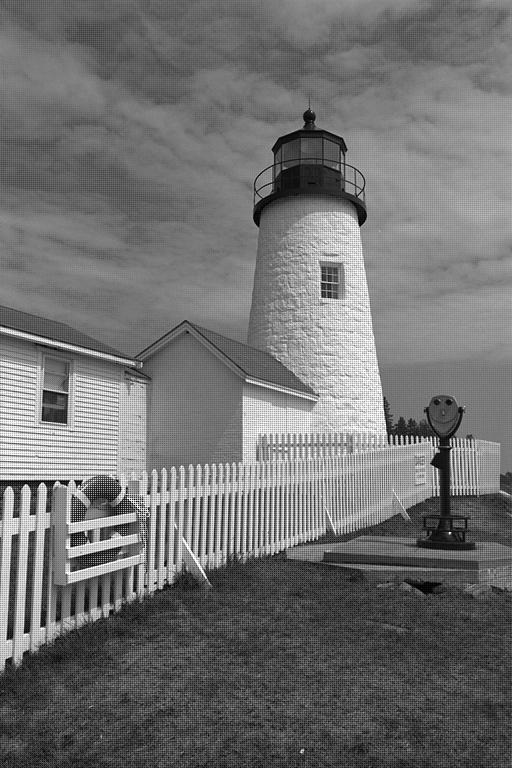
\includegraphics[scale=0.3]{./image/part1-2.png}
\end{figure}

On remarque une différence sur la valeur des pixels si on compare à l'image cfa donnée. Cela est dûe au fait que l'image cfa donnée utilise un filtre différent du notre, un BGB, contrairement à notre solution qui utilise un filtre de type GRG.


\section*{Dématriçage}

Dans cette seconde partie, nous allons implémenter un plugin imageJ qui va permettre de réaliser l'opération de dématrissage d'une image cfa afin de reconstituer l'image originale en filtrant les trois plans de l'image cfa par convolution. Les masques utilisés pour la convolution sont des filtres de Bayer:
\begin{center}
\[
	HR=HB=1/4 \left (
	\begin{array}{ccc}
		1 & 2 & 1\\
        2 & 4 & 2\\
        1 & 2 & 1
	\end{array}
	\right )
\]
\[
	HG=1/4 \left (
	\begin{array}{ccc}
		0 & 1 & 0\\
        1 & 4 & 1\\
        0 & 1 & 0\\ 
	\end{array}
	\right )
\]
\end{center}

Afin de calculer les trois composantes de l'image résultante, on doit appliquer les filtres ci-dessus sur les trois images suivantes:

\begin{figure}[!ht]
	\center
	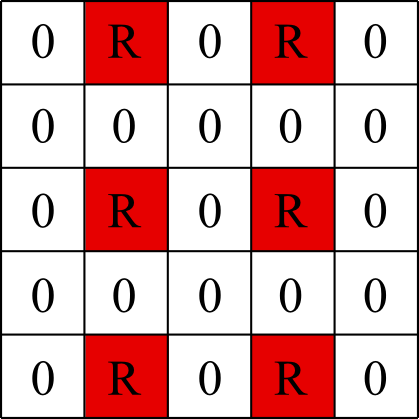
\includegraphics[scale=1.0]{./image/phi_r_cfa_export.png}
	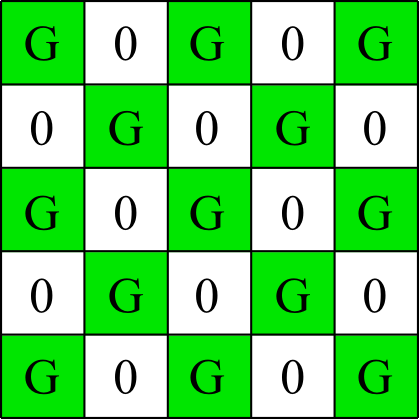
\includegraphics[scale=1.0]{./image/phi_g_cfa_export.png}
	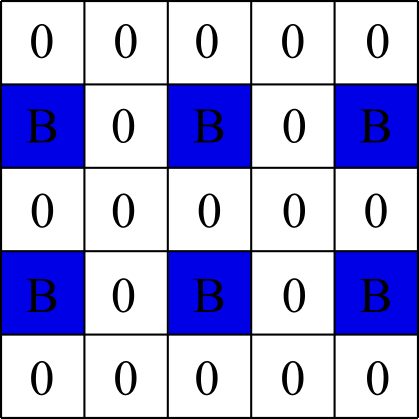
\includegraphics[scale=1.0]{./image/phi_b_cfa_export.png}
\end{figure}

\noindent -Calcul de la composante rouge d'un pixel :\\
Pixel ligne 2 , colonne 2 $\rightarrow$ v(R) = 1/4(1*0+2*R+1*0+2*0+4*0+2*0+1*0+2*R+1*0)=(1/4)*4*R=R\\
Pixel ligne 2 , colonne 3 $\rightarrow$ v(R) = 1/4(1*R+2*0+1*R+2*0+4*0+2*0+1*R+2*0+1*R)=(1/4)*4*R=R\\
Pixel ligne 3 , colonne 4 $\rightarrow$ v(R) = 1/4(1*0+2*0+1*0+2*0+4*R+2*0+1*0+2*0+1*0)=(1/4)*4*R=R\\

\noindent -Calcul de la composante verte d'un pixel :\\
Pixel ligne 2 , colonne 2 $\rightarrow$ v(R) = 1/4(0*G+1*0+0*G+1*0+4*G+1*0+0*G+1*0+0*G)=(1/4)*4*G=G\\
Pixel ligne 2 , colonne 3 $\rightarrow$ v(R) = 1/4(0*0+1*G+0*0+1*G+4*0+1*G+0*0+1*G+0*0)=(1/4)*4*G=G\\


\noindent -Calcul de la composante rouge d'un pixel :\\
Pixel ligne 2 , colonne 2 $\rightarrow$ v(R) = 1/4(1*0+2*0+1*0+2*B+4*0+2*B+1*0+2*0+1*0)=(1/4)*4*B=B\\
Pixel ligne 2 , colonne 3 $\rightarrow$ v(R) = 1/4(1*0+2*B+1*0+2*0+4*0+2*0+1*0+2*B+1*0)=(1/4)*4*B=B\\
Pixel ligne 3 , colonne 4 $\rightarrow$ v(R) = 1/4(1*B+2*0+1*B+2*0+4*0+2*0+1*B+2*0+1*B)=(1/4)*4*B=B\\

Ci-dessus, nous avons récapitulé toutes les combinaisons possibles pour la convolution des pixels et on remarque que pour chaque pixel on obtient une seule valeur pour chaque composante.

\newpage

Nous avons écrit le code qui permet d'obtenir les images correspondant aux trois composantes de l'image cfa; ainsi à partir de ces trois images on peut procéder à l'opération de dématriçage qui permet de reconstituer l'image originale. L'image de gauche correspond à la composante rouge, l'image du milieu à la composante verte et l'image de droite à la composante bleue.
\begin{figure}[!ht]
\center
	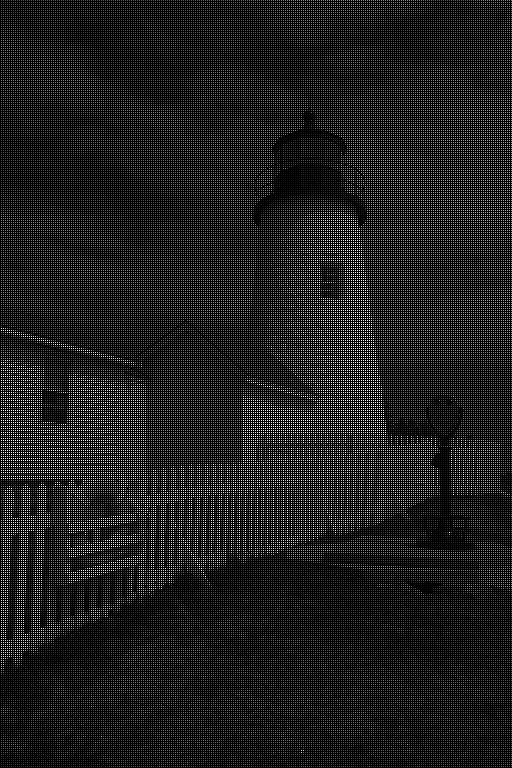
\includegraphics[scale=0.3]{./image/part2-23Rouge.png}
	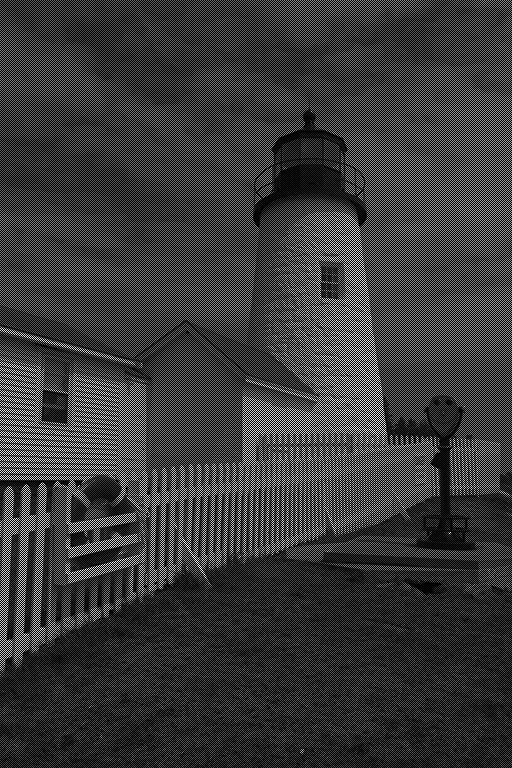
\includegraphics[scale=0.3]{./image/part2-23Vert.png}
	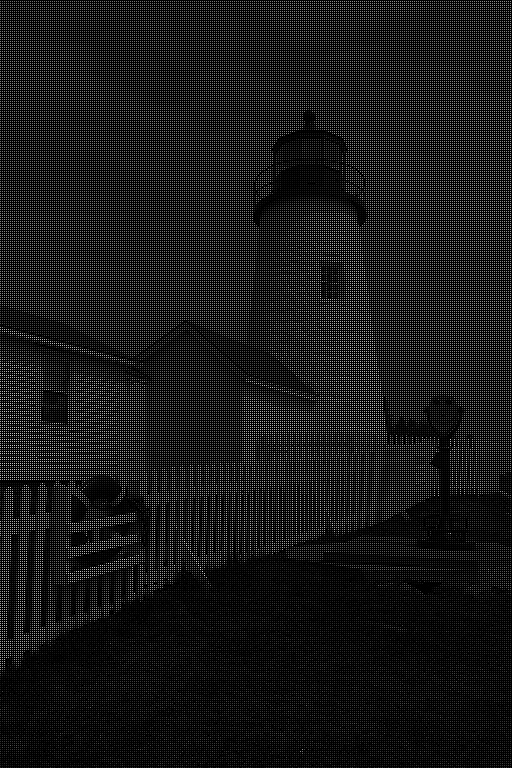
\includegraphics[scale=0.3]{./image/part2-23Bleu.png}
\end{figure}

Voici le code permettant d'obtenir ces résultats: 

\begin{lstlisting}[style=Java]
public ImageProcessor  cfa_samples(ImageProcessor imp, int row_order) {
		width = imp.getWidth();
		height = imp.getHeight();
		ImageProcessor composante_imp = new ByteProcessor(width,height);
		for(int j=0; j<height;j++){
			for(int i=0; i<width ;i++){
				// Les modulos permettent de calculer le deplacements du filtres selon les couleurs
				if(row_order==0)
					if(j%2==0 && i%2==1)
						composante_imp.putPixel(i,j,imp.getPixel(i,j));
				if(row_order==1)
					if((j+i)%2==0)
						composante_imp.putPixel(i,j,imp.getPixel(i,j));
				if(row_order==2)
					if(j%2==1 && i%2==0)
						composante_imp.putPixel(i,j,imp.getPixel(i,j));	
		}			
	}		
	return composante_imp;
}
\end{lstlisting}

\newpage

A partir des images ci-dessus, nous allons reconstruire une image couleur correspondant à l'image originale à partir de laquelle on a généré l'image cfa. Cependant, l'image obtenue contient des défauts notamment au niveau des barrières qui sont jaunes/bleues. Ceci est en fait du au calcul des composantes couleurs par interpolation bilinéaire.

\begin{figure}[!ht]
	\center
	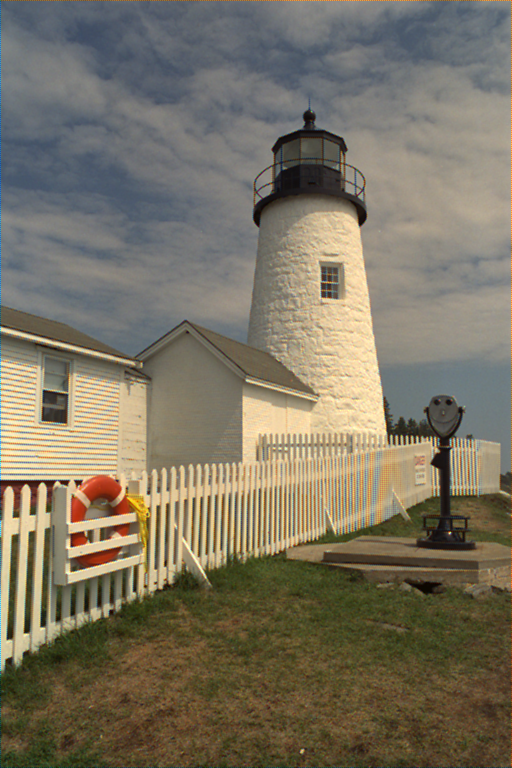
\includegraphics[scale=0.3]{./image/part2-4.png}
\end{figure}

Étant donnée que l'interpolation bilinéaire ne permet pas d'obtenir des résultats super plausibles, nous allons procéder au dématriçage par une autre approche qui se base sur l'estimation locale d'un gradient. Comme vu dans le cours, cette méthode permettra d'obtenir un résultat plus correcte.

\section*{Dématriçage basé sur l'estimation locale d'un gradient} 

Dans cette partie nous utiliserons l'algorithme de dématricage proposé par Hamilton $\&$ Adams. Nous allons calculer la composante verte de la cfa avec cet algorithme et la composante rouge et verte avec l'interpolation bilinéaire.

Nous avons complété le run et le setup (très ressemblant aux classes précédement complétées) de la facon suivante:
\begin{lstlisting}[style=Java]
	public int setup(String arg, ImagePlus imp) {
		this.imp = imp;
		return compute_cfa.DOES_RGB;
	}

	public void run(ImageProcessor ip) {
		// Lecture des dimensions de la fenetre
		width = imp.getWidth();
		height = imp.getHeight();

		// Dispositions possibles pour le CFA
		String[] orders = {"R-G-R", "B-G-B", "G-R-G", "G-B-G"};

		// Definition de l'interface
		GenericDialog dia = new GenericDialog("Generation de l'image CFA...", IJ.getInstance());
		dia.addChoice("Debut de premiere ligne :", orders, orders[2]);
		dia.showDialog();

		// Lecture de la reponse de l'utilisateur
		if (dia.wasCanceled()) return;
		int order = dia.getNextChoiceIndex();

		// Generation de l'image CFA
		ImageProcessor cfa = this.cfa(order);
		this.imp = new ImagePlus("calcul cfa", cfa);
		imp.show();

		//creation des composantes RB bilineaire et G en Hamilton
		ImageProcessor  r = cfa_samples(cfa ,0);
		ImageProcessor  g = est_G_hamilton(cfa);
		ImageProcessor  b = cfa_samples(cfa ,2);

		float[] hrb = {0.25f,0.5f,0.25f, 0.5f,1.0f,0.5f, 0.25f,0.5f,0.25f};// RED and BLUE
		float[] hg ={0.0f,0.25f,0.0f, 0.25f,1.0f,0.25f,0.0f,0.25f,0.0f	}; // GREEN
		
		Convolver convolve = new Convolver();
		convolve.setNormalize(false);
		convolve.convolve(r,hrb,3,3);				
		convolve.convolve(b,hrb,3,3);
		
		// Calcul des echantillons de chaque composante de l'image CFA
		ImageStack samples_stack = imp.createEmptyStack();
		samples_stack.addSlice("rouge", r);	// Composante R
		samples_stack.addSlice("vert", g);// Composante G
		samples_stack.addSlice("bleu", b);	// Composante B
		ImagePlus cfa_samples_imp = imp.createImagePlus();
		cfa_samples_imp.setStack("echantillons couleur CFA", samples_stack);
		cfa_samples_imp.show();
	}
\end{lstlisting}

La méthode Hamilton, étant longue, est fournie dans le listing à la fin de ce document.

Nous obtenons les trois images comme précédemment, rouge, verte et bleu. Nous remarquons que l'image verte présente ci-dessous (obtenue avec l'algorithme de Hamilton) n'est pas floutée puisqu'elle n'a pas subit la convolution, ce qui est un plus comparé à l'interpolation bilinéaire. 

\begin{figure}[!ht]
	\center
	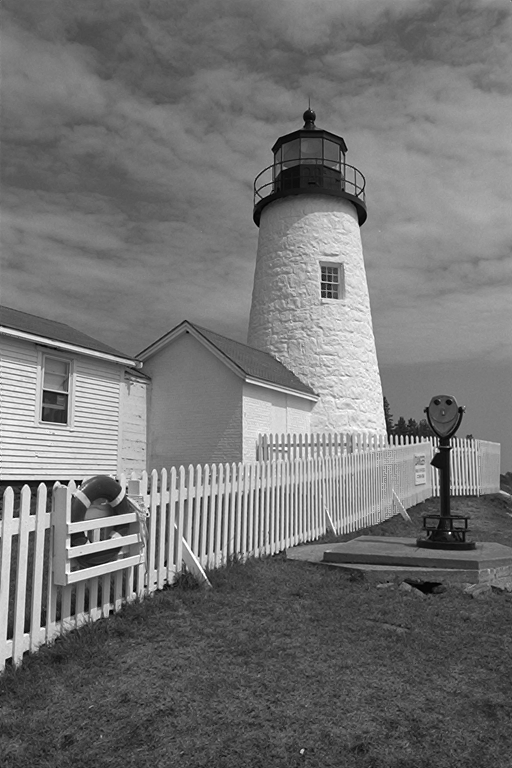
\includegraphics[scale=0.3]{./image/part3-31Vert.png}
\end{figure}

\newpage

Une fois les trois images regroupées nous obtenons l'image suivante:

\begin{figure}[!ht]
	\center
	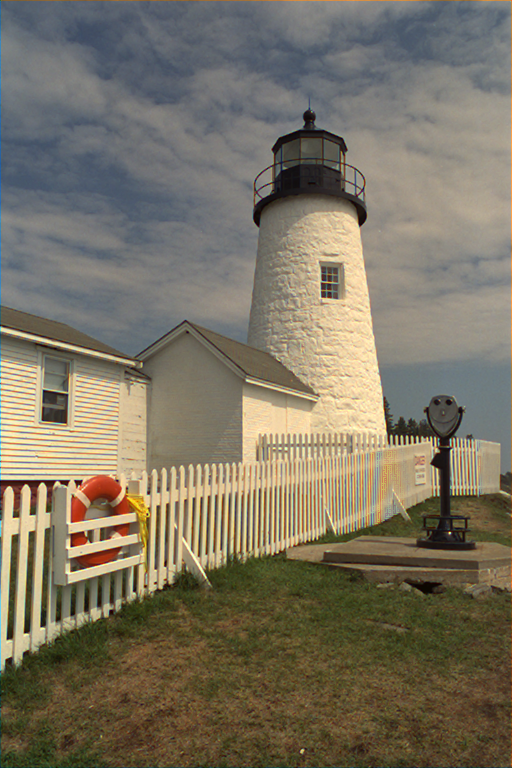
\includegraphics[scale=0.4]{./image/part3-31.png}
	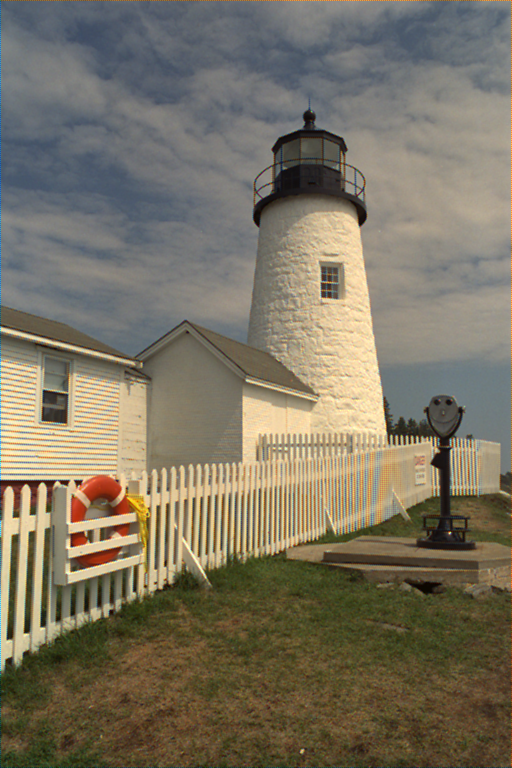
\includegraphics[scale=0.4]{./image/part2-4.png}
\end{figure}

Le résultat obtenu présente une "déformation" sur les barrières du fond. Cette "déformation" était attendue puisqu'elle correspond à un résultat obtenu avec la méthode du gradient (cf, image du cours). En comparant avec l'image de gauche, qui correspond au résultat de la partie de contenant uniquement de l'interpolation bilinéaire, on observe que l'image avec la méthode de gradient sur la composante verte est de meilleur qualité.

En effet on observe que certains effet "jaune/bleu" s'atténuent. Mieux encore, l'effet "pixélisé/saccadé" apparaisant sur le phar, les maisons ... disparaît.

L'image est donc de meilleur qualité mais appliqué la méthode du gradient sur les composantes rouge et bleu aurait pour résultat une image de meilleur qualité.
 	
\section*{Conclusion}

En conclusion on peut dire que nous avons observé la différence entre la méthode d'interpolation bilinéaire et la méthode du gradient. La méthode d'interpolation linéaire nous permet d'obtenir avec peu de calcul une image de qualité moyenne (passable pour un format d'image dit avec perte de qualité). La méthode du gradient permet d'obtenir une image de meilleur qualité mais effectue plus de calcul. Une image de grande dimension pourrait permettre de constater la différence de temps de calcul entre les deux méthodes.

\newpage

\section*{Listing}


\begin{lstlisting}[style=Java]
/**
 * My_Plugin_.java 
 * @  Douaille Erwan - Nait Abdelaziz Yanis
 *
 */
import ij.*;
import ij.plugin.filter.*;
import ij.process.*;
import ij.gui.*;

public class demat_ha implements PlugInFilter {

	ImagePlus imp;	// Fenetre contenant l'image de reference
	int width;		// Largeur de la fenetre
	int height;		// Hauteur de la fenetre

	public int setup(String arg, ImagePlus imp) {
		this.imp = imp;
		return compute_cfa.DOES_RGB;
	}

	public void run(ImageProcessor ip) {

		// Lecture des dimensions de la fenetre
		width = imp.getWidth();
		height = imp.getHeight();

		// Dispositions possibles pour le CFA
		String[] orders = {"R-G-R", "B-G-B", "G-R-G", "G-B-G"};

		// Definition de l'interface
		GenericDialog dia = new GenericDialog("Generation de l'image CFA...", IJ.getInstance());
		dia.addChoice("Debut de premiere ligne :", orders, orders[2]);
		dia.showDialog();

		// Lecture de la reponse de l'utilisateur
		if (dia.wasCanceled()) return;
		int order = dia.getNextChoiceIndex();


		// Generation de l'image CFA
		ImageProcessor cfa = this.cfa(order);
		this.imp = new ImagePlus("calcul cfa", cfa);
		imp.show();

		//creation des composantes RB bilineaire et G en Hamilton
		ImageProcessor  r = cfa_samples(cfa ,0);
		ImageProcessor  g = est_G_hamilton(cfa);
		ImageProcessor  b = cfa_samples(cfa ,2);

		float[] hrb = {0.25f,0.5f,0.25f, 0.5f,1.0f,0.5f, 0.25f,0.5f,0.25f};// RED and BLUE
		float[] hg ={0.0f,0.25f,0.0f, 0.25f,1.0f,0.25f,0.0f,0.25f,0.0f	}; // GREEN


		Convolver convolve = new Convolver();
		convolve.setNormalize(false);
		
		convolve.convolve(r,hrb,3,3);				
		convolve.convolve(b,hrb,3,3);
		
		// Calcul des echantillons de chaque composante de l'image CFA
		ImageStack samples_stack = imp.createEmptyStack();

		samples_stack.addSlice("rouge", r);	// Composante R
		samples_stack.addSlice("vert", g);// Composante G
		samples_stack.addSlice("bleu", b);	// Composante B

		ImagePlus cfa_samples_imp = imp.createImagePlus();
		cfa_samples_imp.setStack("Echantillons couleur CFA", samples_stack);
		cfa_samples_imp.show();

	}

	public ImageProcessor cfa(int row_order) {
		// Image couleur de reference et ses dimensions
		ImageProcessor ip = imp.getProcessor();
		width = imp.getWidth();
		height = imp.getHeight();

		int pixel_value = 0;	// Valeur du pixel source
		ImageProcessor cfa_ip = new ByteProcessor(width,height);	// Image CFA generee

		// echantillons G
		for (int y=0; y<height; y+=2) {
			for (int x=0; x<width; x+=2) {
				pixel_value = ip.getPixel(x,y);
				int green = (int)(pixel_value & 0x00ff00)>>8;
			cfa_ip.putPixel(x,y,green);
			}
		}
		for (int y=1; y<height; y+=2) {
			for (int x=1; x<width; x+=2) {
				pixel_value = ip.getPixel(x,y);
				int green = (int)(pixel_value & 0x00ff00)>>8;
			cfa_ip.putPixel(x,y,green);
			}
		}
		// echantillons R
		for (int y=0; y<height; y+=2) {
			for (int x=1; x<width; x+=2) {
				pixel_value = ip.getPixel(x,y);
				int red = (int)(pixel_value & 0xff0000)>>16;
			cfa_ip.putPixel(x,y,red);
			}
		}
		// echantillons B
		for (int y=1; y<height; y+=2) {
			for (int x=0; x<width; x+=2) {
				pixel_value = ip.getPixel(x,y);
				int blue = (int)(pixel_value & 0x0000ff);
				cfa_ip.putPixel(x,y,blue);
			}
		}

		return cfa_ip;
	}


	public ImageProcessor  cfa_samples(ImageProcessor imp, int row_order) {
		width = imp.getWidth();
		height = imp.getHeight();
		ImageProcessor composante_imp = new ByteProcessor(width,height);
		for(int j=0; j<height;j++){
			for(int i=0; i<width ;i++){
				if(row_order==0)
					if(j%2==0 && i%2==1)
						composante_imp.putPixel(i,j,imp.getPixel(i,j));
				if(row_order==1)
					if((j+i)%2==0)
						composante_imp.putPixel(i,j,imp.getPixel(i,j));
				if(row_order==2)
					if(j%2==1 && i%2==0)
						composante_imp.putPixel(i,j,imp.getPixel(i,j));	
			}			
		}		
		return composante_imp;
	}
	
	ImageProcessor est_G_hamilton(ImageProcessor cfa_ip) {
		width = cfa_ip.getWidth();
		height = cfa_ip.getHeight();
    		ImageProcessor est_ip = cfa_ip.duplicate();
    		for(int j=0;j<height;j=j+2){
    			for(int i=1;i<width;i=i+2){
    			
    				int pCourant = cfa_ip.getPixel(i,j) & 0xff;
    				
    				int pXGauche = cfa_ip.getPixel(i-1,j) & 0xff;
    				int pXDroite = cfa_ip.getPixel(i+1,j) & 0xff;
    				int pXGaucheG = cfa_ip.getPixel(i-2,j) & 0xff;
    				int pXDroiteD = cfa_ip.getPixel(i+2,j) & 0xff;
    				
    				int pYHaut = cfa_ip.getPixel(i,j-1) & 0xff;
    				int pYBas = cfa_ip.getPixel(i,j+1) & 0xff;
    				int pYHautH = cfa_ip.getPixel(i,j-2) & 0xff;
    				int pYBasB = cfa_ip.getPixel(i,j+2) & 0xff;
    				
    				int gradX= Math.abs(pXGauche-pXDroite)+Math.abs(2*pCourant-pXGaucheG-pXDroiteD);
    				int gradY= Math.abs(pYHaut-pYBas)+Math.abs(2*pCourant-pYHautH-pYBasB);
    				if(gradX<gradY){
    					
    					est_ip.putPixel(i,j,((pXGauche+pXDroite)/2+(2*pCourant-pXGaucheG-pXDroiteD)/4));
    				}
    				else if(gradX>gradY){
    					est_ip.putPixel(i,j,((pYHaut+pYBas)/2+(2*pCourant-pYHautH-pYBasB)/4));
    				}
    				else{
    					est_ip.putPixel(i,j,((pYHaut+pXGauche+pXDroite+pYBas)/4+(4*pCourant-pYHautH-pXGaucheG-pXDroiteD-pYBasB)/8));
    				}
    			}
    		}
    		
    		for(int j=1;j<height;j=j+2){
    			for(int i=0;i<width;i=i+2){
    			
    				int pCourant = cfa_ip.getPixel(i,j) & 0xff;
    				
    				int pXGauche = cfa_ip.getPixel(i-1,j) & 0xff;
    				int pXDroite = cfa_ip.getPixel(i+1,j) & 0xff;
    				int pXGaucheG = cfa_ip.getPixel(i-2,j) & 0xff;
    				int pXDroiteD = cfa_ip.getPixel(i+2,j) & 0xff;
    				
    				int pYHaut = cfa_ip.getPixel(i,j-1) & 0xff;
    				int pYBas = cfa_ip.getPixel(i,j+1) & 0xff;
    				int pYHautH = cfa_ip.getPixel(i,j-2) & 0xff;
    				int pYBasB = cfa_ip.getPixel(i,j+2) & 0xff;
    				
    				int gradX= Math.abs(pXGauche-pXDroite)+Math.abs(2*pCourant-pXGaucheG-pXDroiteD);
    				int gradY= Math.abs(pYHaut-pYBas)+Math.abs(2*pCourant-pYHautH-pYBasB);
    				if(gradX<gradY){
    					
    					est_ip.putPixel(i,j,((pXGauche+pXDroite)/2+(2*pCourant-pXGaucheG-pXDroiteD)/4));
    				}
    				else if(gradX>gradY){
    					est_ip.putPixel(i,j,((pYHaut+pYBas)/2+(2*pCourant-pYHautH-pYBasB)/4));
    				}
    				else{
    					est_ip.putPixel(i,j,((pYHaut+pXGauche+pXDroite+pYBas)/4+(4*pCourant-pYHautH-pXGaucheG-pXDroiteD-pYBasB)/8));
    				}
    			}
    		}
    		
    		return (est_ip);
	}
}
\end{lstlisting}

\end{document}